\documentclass[../../course]{subfiles}

\renewcommand\thesection{\arabic{section}}


\begin{document}

\section{Generating Complex Sequences} \label{sec:wrkGenCompSeqs}

In section \ref{lst:threeSeqs} we generated three signals with three different
frequencies. The important thing to notice is that, they all are real valued
sequences. In this section, we will see how we can combine\footnote{as real and
imaginary part of a complex sequence} these signals into \emph{complex} sequences.

\subsection{Mixing of Signals}

We have three different distinct sequences, so how we can mix these signals into
more diverse \emph{complex} sequences ? This can be simply done by taking one of our
\emph{real valued} sequence as the \emph{real part} of the \emph{complex} sequence
and another \emph{real valued} sequence as the \emph{imaginary part} of the
\emph{complex} sequence. By doing so, one may encounter that there are many ways
to arrange these sequences. Or so to say, there are many different combinations\footnote{of
different real and imaginary sequences}, thus generating there many distinct \emph{complex}
sequences.


\begin{figure} [H]

    \centering

    \begin{tabularx} {\textwidth} {
            *{3}{>{\centering\arraybackslash}X}
        }

        & & \\

        \adjustbox{max width = 0.3\textwidth} {
            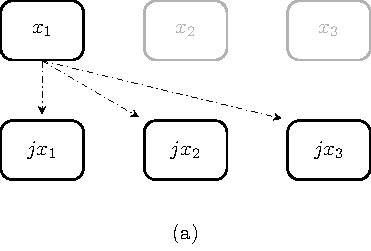
\includegraphics[height = 0.3\textheight] {tikzpics/epicCplxCombFirst.pdf}
        }

        &

        \adjustbox{max width = 0.3\textwidth} {
            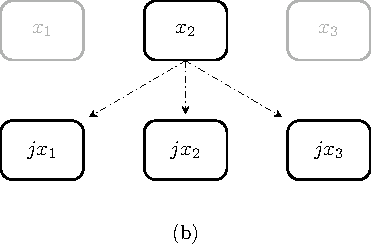
\includegraphics[height = 0.3\textheight] {tikzpics/epicCplxCombSecond.pdf}
        }

        &

        \adjustbox{max width = 0.3\textwidth} {
            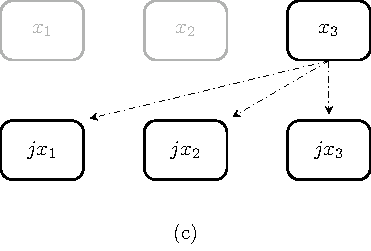
\includegraphics[height = 0.3\textheight] {tikzpics/epicCplxCombThird.pdf}
        }

        \\

        \captionof{figure} {
            Taking $x_{1}$ as real part and $x_{1}$, $x_{2}$, and $x_{3}$ as imaginary parts.
        }
        \label{fig:cplxCombFirst}

        &

        \captionof{figure} {
            Taking $x_{2}$ as real part and $x_{1}$, $x_{2}$, and $x_{3}$ as imaginary parts.
        }
        \label{fig:cplxCombSecond}

        &

        \captionof{figure} {
            Taking $x_{3}$ as real part and $x_{1}$, $x_{2}$, and $x_{3}$ as imaginary parts.
        }
        \label{fig:cplxCombThird}

    \end{tabularx}

\end{figure}

As we can see from figures \ref{fig:cplxCombFirst} to \ref{fig:cplxCombThird} there is a
total of $3 \times 3 = 9$ different ways to combine these three signals. In the upcoming
subsections we will see each of these combinations in detail.

\begin{figure} [H]
    \centering
    \renewcommand{\arraystretch}{1}

    \begin{tabularx} {\textwidth} {
            *{1}{>{\centering\arraybackslash}X}
            *{1}{>{\centering\arraybackslash}m{0.3\textwidth}}
        }

        { \begin{tabularx} {0.65\textwidth} {
                    *{4}{>{\centering\arraybackslash}X}
                }
                \toprule
                \textsc{Combination Name} & \textsc{Real Part} & \textsc{Imaginary Part} & \textsc{Complex Sequence} \\
                \midrule
                \textsc{Comb A} & $x_{1}$ & $x_{1}$ & $x_{1} + j x_{1}$  \\
                \textsc{Comb B} & $x_{1}$ & $x_{2}$ & $x_{1} + j x_{2}$  \\
                \textsc{Comb C} & $x_{1}$ & $x_{3}$ & $x_{1} + j x_{3}$  \\
                \cmidrule(lr){1-4}
                \textsc{Comb E} & $x_{2}$ & $x_{2}$ & $x_{2} + j x_{2}$  \\
                \textsc{Comb D} & $x_{2}$ & $x_{1}$ & $x_{2} + j x_{1}$  \\
                \textsc{Comb F} & $x_{2}$ & $x_{3}$ & $x_{2} + j x_{3}$  \\
                \cmidrule(lr){1-4}
                \textsc{Comb G} & $x_{3}$ & $x_{1}$ & $x_{3} + j x_{1}$  \\
                \textsc{Comb H} & $x_{3}$ & $x_{2}$ & $x_{3} + j x_{2}$  \\
                \textsc{Comb I} & $x_{3}$ & $x_{3}$ & $x_{3} + j x_{3}$  \\
                \bottomrule
            \end{tabularx} }

            &

            \captionof {table} {
                Different combinations of \emph{Complex Sequences} and there respective
                \emph{Real} and \emph{Imaginary} parts.
            }

            \\

    \end{tabularx}


\end{figure}

\subsection{Gen}

%% \begin{figure}
%%     \centering
%%     \adjustbox{max width = \textwidth} {
%%         \includegraphics[height = 0.8\textheight] {tikzpics/testing.pdf}
%%     }
%%     \captionof{figure} {Testing}
%%     \label{plt:testing}
%% \end{figure}
%%
%%
%% \begin{figure}
%%     \centering
%%     \adjustbox{max width = 0.7\textwidth} {
%%         \includegraphics[height = 0.8\textheight] {tikzpics/hai.pdf}
%%     }
%%     \captionof{figure} {Ahai}
%%     \label{plt:wowo}
%% \end{figure}
%%
%%
%%
%% \begin{figure}
%%     \centering
%%     \adjustbox{max width = 0.7\textwidth} {
%%         \includegraphics[height = 0.8\textheight] {tikzpics/woo.pdf}
%%     }
%%     \captionof{figure} {Ahai}
%%     \label{plt:wowo}
%% \end{figure}





\end{document}
